\chapter{The Missing Baryon Problem}
	%  - Missing Baryon Problem
			%-  Stellar Baryons
			%- 	Cold Interstellar Medium
			%- 	Residual Lyman Alpha 
			%- 	OVI and BLA Absorbers
			%- 	Hot Gas in Clusters 
	%	- Warm Hot Intergalactic Medium
	%  	- Sunayev-Zeldovich Effect
			%-	Atomic Physics
			%- 	Signal in CMB 

The Missing Baryon problem is that we see more baryons at high redshift, than at low redshift. At high redshift ($z>2$), the Lyman-$\alpha$ forest provides a good measure of the proportion of baryons, since at these redshifts the majority of baryons in the universe are contained in diffuse, low-density gas. These analyses give a reported value 
$$\Omega_{b} \geq 0.035 $$ 

Observed light-element ratios and standard nucleosynthesis allows for direct computation of the expected baryon densities, which is in agreement with the above figure \citep{1998sese.conf..113B}
$$\Omega_{b} = (0.019\pm 0.001)h^{-2} = 0.039 \pm 0.002 $$

The $\sim 2-3 \sigma$ agreement between these two measures of baryon density, and the measurement obtained from the CMB ($\Omega_{b} = (0.0224 \pm 0.0001) h^{-2}$) lends confidence to the value obtained by Planck. The CMB measurement is far more precise than the other measurements due to it requiring inherently fewer assumptions, and so the systematics for a CMB measurement are often much easier to quantify. 

\par However, at low redshifts, all analysis indicates that the summing over all observed contributions gives a value of 

$$\Omega_\star + \Omega_{HI} + \Omega_{H_2} + \Omega_{X-Ray,cl} \approx 0.0068 \leq 0.011, $$

where $\Omega_\star$ refers to the density of stars, $\Omega_{HI}$ is the density of neutral hydrogen, $\Omega_{H_2}$ is the density of molecular hydrogen, and $\Omega_{X-Ray,cl} $ is the density derived from X ray sources, and other measurements of clusters.
\par This severe discrepency between measurements at high and low redshifts suggests that either the majority of the baryons at low redshifts are yet to be detected, there are fundamental errors in numerous independent measures of the baryon density at high redshift, or there is yet-to-be uncovered new physics. Occams razor suggests that new physics is unlikely, given how self-consistent both sets of measurement are, and the agreement between independent high redshift measurements, such as the Lyman $\alpha$ forest, and the CMB, suggests that the most likely problem is that we have not made an accurate account of baryons in the local universe.

\section{A Census of Baryons at Low Redshift}
\subsection{Stellar Baryons}
The most obvious location to search for baryons are in the stellar populations of galaxies. At a broad level, we can imagine that there are two distinct stellar populations which can be considered to be found in high density galaxies; a class of old stars which exists in the bulge of a galaxy ($\Omega_{\star,\text{Bulge}}$), and a class of young stars in the disk ($\Omega_{\star,\text{Disk}} $), as well as a third population existing in irregular galaxies ($\Omega_{\star,\text{Irr}}$).

\par Estimating the proportion of stellar baryons therfore becomes an exercise in galactic morphology and luminosity density function computation. Perfoming this calculation gives mean mass density numbers for these three classes of stars of
\begin{align*}
\Omega_{\star,\text{Bulge}} &= (0.00180^{+0.00121}_{-0.00085}) h^{-1} \\
\Omega_{\star,\text{Disk}} &= (0.00060^{+0.00030}_{-0.00024}) h^{-1} \\
\Omega_{\star,\text{Irr}} &= (0.000048^{+0.000033}_{0.000026}) h^{-1}
\end{align*}

These numbers depend on the mass-to-light ratio for age estimation, and so in turn are dependant on the cosmological parameters in a complex way. Even if efforts were made to remove this dependancy by changing the methodology used to calculate the mass-to-light function, the necessity for the new methodology to hold consistent with other measurements would force the dependancy regardless.

\subsection{Cold Interstellar Medium}
We also know that some of the baryons in the local universe are stored in the cold interstellar medium, a term for neutral and molecular gas, primarily consisting of unionised hydrogen (HI). The HI present in gas-rich galaxies is the best tracer for the neutral hydrogen mass content in the near universe, since it can be shown that very little neutral gas is present in objects outside the galaxy population in these regions. At redshift $z \approx 0$, there have not been any free HI clouds detected by radio surveys that have not yet subsequently been detected in optical bands \citep{1993ApJ...419..515R}, and so optical detection in galaxies can be considered to be adequate when taking a census of the total baryons contained in the cold interstellar medium. 
\par The HI content of a given galaxy can be calculated from the optical luminosity functions of given galaxy morphological types. For a given optical luminosity function $\phi^T(M)$, and a given HI mass content $M_{HI}^T(M)$, as functions of absolute magnitude $M$, the total HI mass content of a given galaxy morphological type $T$ can be found by computing an integral over all luminosities
$$M_{HI} = \int \phi^T(M) M_{HI}^T(M) dM $$

Adding all the contributions for all morphological types will therefore give an estimate of the total HI at $z=0$. At these distances, spiral galaxies are the primary contributors to the neutral hydrogen content, containing $\sim 89\%$ of the hydrogen mass. Initial estimates \citep{1993ApJ...419..515R} place the mass density of neutral hydrogen at the present time at 

$$\Omega_{HI} = (2.5 \pm 0.6) \times 10^{-4} h_{75}^{-1} $$

Later surveys, such as the HI Parkes All-Sky Survey (HIPASS), refined this measurement further \citep{2003AJ....125.2842Z}. HIPASS is a blind survey of the southern sky south consisting of approximately 7000 galaxies. The much higher number of galaxies in this survey necessitated a different method of computing the neutral hydrogen fraction. Taking a statistical approach the probability that a galaxy with a given HI mass is
$$ p(M_{HI,i}|D) = \frac{\theta(M_{HI,i})}{\int_{M_{HI,\lim(D_i)}}^\infty \theta(M_{HI}) dM_{HI}}, $$
where $M_{HI,\lim(D_1)}$ is the minimum detectable HI mass at some distance $D_i$. This essentially gives the fraction of galaxies in the survey with a given HI mass sufficient to be detected. The parent distribution $\theta$ can then be maximised by finding which product of probabilities is also maximal. The statistical nature of this method requires accounting for various forms of bias, such as selection bias in the survey, the Eddington effect, self-absorption of the neutral hydrogen, and cosmic variance. This methodology gives a measure of the mass density as 
$$\Omega_{HI} = (3.8 \pm 0.6) \times 10^{-4} h_{75}^{-1} $$
\subsection{Quasar Absorbers}
\subsubsection{Photoionised Lyman $\alpha$}
At higher redshifts, essentially the entirety of the baryon content in the universe can be found in large quanties of gas that have not yet collapsed into galaxies, which shows up very clearly in the Lyman $\alpha$ (Ly$\alpha$) forest. 
\par The Lyman $\alpha$ forest is a series of absorption lines that are visible in the spectra of distant quasars, which intersect with clouds of neutral hydrogen along their line of sight to us. Since the light emmitted by the quasar passes through many hydrogen clouds, and is redshifted by cosmological expansion, there will be a characteristic absorption signal in the spectrum which corresponds to the position of the clouds relative to the quasar. These absorption signals make the Quasar spectrum look like a forest, hence, the name Lyman $\alpha$ forest. 

\par At low redshifts, we can search for the residual Ly$\alpha$ signal using HI absorber frequencies in distant quasars. By making the assumption that these absorbers are isothermal spheres, and choosing a given impact parameter, the total cloud mass can be essentially inferred from the HI column density. 

\par One model for estimating the contribution of the local Lyman $\alpha$ forest is outlined by \cite{2000ApJ...544..150P}. From big bang nucleosynthesis, the total baryons contributed from the low-$z$ Ly$\alpha$ is given by 
$$\Omega_{Ly\alpha} = \int_{N_{min}}^{N_{max}} \frac{ \phi_0(N_{HI},p) M_{cl}(N_{HI}, p, J_0)}{\rho_{crit}} dN_{HI} ,$$
where $M_{cl}(N_{HI}, p, J_0)$ is the mass of an individual cloud , $\phi_0(N_{HI},p)$ is space density of the clouds, $N_{HI}$ is the column density of the clouds, $J_0$ is the specific intensity of the metagalactic ionizing radiation field, $\rho_{crit} = 3 H_0^2/8 \pi G $ is the critical density at the present day which is necessary to maintain flatness.

\par Making more assumptions about the compostion of the spheres, and that the gas is in photoionising equilibrium, and the impact parameter, this reduces the integral to
$$\Omega_{Ly\alpha} = (0.008 \pm 0.001) \left[ J_{-23} p_{100} \left(\frac{ 4.8}{ \alpha_s + 3} \right) \right]^{1/2} h_{70}^{-1}, $$
where $\alpha_s$ is the spectral index of the radiation field, $J_{-23}= J_0/10^{-23}$, $p_{100} = p/(\SI{100}{\kilo\parsec})$ and $h_{70} = H_0/(\SI{70}{\mega\parsec})$ . This corresponds to approximately $20\%$ of the baryons, but it inherently makes a number of rather significant assumptions, which are highly dependant on the number of Lyman $\alpha$ absorbers detected at low redshifts. 
\par Further accounting for the fact that the clouds are gravitationally bound, and that their densities are typical over a characteristic Jeans length allows for further refinement of this number \citep{2001ApJ...559..507S}. Doing so yields a measure of the number of baryons in the residual Lyman $\alpha$ forest of $\Omega_{Ly\alpha} = 29 \% \pm 4\%$ \citep{ 2004ApJS..152...29P,2008ApJ...679..194D}  
\subsubsection{OVI and BLA Absorbers}

Because gas at low redshift exists at a large range of temperatures, and at a higher metalicity than the same gas at higher redshifts, distant quasars will exhibit absorption from higher Lyman alpha lines, such as oxygen (OVI), and broad Lyman $\alpha$ lines (BLA). The OVI absorption line probes gas in temperature ranges from $10^5$ - $10^6$ K, which has been shock heated as a result of gravitational instability during structure formation. Gas hotter than this is only sensitive to very weak absorption lines from higher ions, such as OVII, OVIII, NeX, NVI, and NVII, which are only detectable in weak X-Rays \citep{2005ApJ...624..555D}. 
\par Broad Lyman $\alpha$ also act as a tracer of the gas in these temperature ranges. Theory suggests that the ionisation equilibrium of gas should contain a very small portion of neutral gas, typically $f \sim 10^{-5} - 10^{-6}$, so there should be some Ly $\alpha$ emission, thermally broadened by the intervening gas \citep{2006A&A...445..827R}. It is not entirely clear if the OVI and BLA absorbers trace the same underlying gas phase, so they have been included here together. 
\par The method of calculating these numbers is a comparatively simply integral, over the number of absorbers per redshift bin. This does make several assumptions which are sensitive to the visibility, as well as the number of absorbers in a given survey. \par \cite{2005ApJ...624..555D} found the proportion of matter contained in OVI absorbers to be approximately $5\%$, extrapolated from $\sim 50$ absorbers. However, this number is highly dependant on the model chosen to describe the spread of oxygen/hydrogen metalicities, the redshift range of the survey, and OVI ionisation fractions, leading to large errors on this measurement. 
\par \cite{2006A&A...445..827R} found the proportion from BLAs to be $\sim 15 \% - 150 \%$ of the total baryon fraction, from a sample of between 20 and 50 sources. The reason for the large uncertainty is the inherent uncertainty in the detection of BLA sources. In fact, the unreasonably high measurement of the baryon fraction says that this method is inherently counting sources which are not actually good tracers of the free baryons. There is also some confusion regarding sources which appear as both OVI and BLA absorbers, since the connection between the two types is not clear. 

\subsection{Summary}

These methods all carry some sources of error with them, some so large that they call into question their validity entirely. Calculations of stellar baryons and cold interstellar medium are limited by the brightness that a given survey instrument is sensitive to, and so real world considerations like integration time, survey depth, and survey area make using them as an accurate measure difficult. The limiting factor for absorption studies is the incredibly low number of observed absorbers. The areas of phase space that absorption studies probe contains requires bright sources such as quasars to align with intervening matter. This low likelihood, and the unknowns associated with models of the source behaviour makes this a vague probe of the baryon fraction at best. There is also the very real possibility that they probe the same phase space of baryons, leading to an unknown level of degeneracy in the overall baryon fraction. 

\par If we include some smaller contributions, such as from cluster contributions ($\Omega_b^{(cl)} \sim 4 \%$)\citep{2004ApJ...616..643F}, or the circumgalactic medium ($\Omega_b^{(CGM)} \sim 5 \% \pm 3\%$), these still do not account for the entirety of the baryon component known from the CMB. Some revised estimates of the total baryon content at low redshift considered that the limitations of observations were primarily to blame for the discrepency, and not inherently new physics \citep{1994MNRAS.267...13B, 1998ApJ...503..518F}.

\par If we examine the latest estimates of the local baryon content in its entirety by \cite{2012ApJ...759...23S}, shown in Table \ref{table:baryon_census}, it becomes clear that up to $30 \%$ of the universe's baryons are not being located by direct observational methods.

\begin{table}[h!]
\centering
\begin{tabular}{||c c c||} 
 \hline
 Source & $\Omega_b$ Percentage & Error \\
 \hline\hline
 Photoionised Lyman $\alpha$ Forest & $28\%$ & $\pm 11 \%$ \\
 \hline
 X Ray Absorbers (OVI and BLA) & $31\%$ & $\pm 11 \%$ \\
 \hline
 Galaxies & $7\%$ & $\pm 2\%$ \\
 \hline
 Circumgalactic Medium  & $5\%$ & $\pm 3 \%$  \\
 \hline
 Intercluster Medium  & $4\%$ & $\pm 1.5 \%$ \\
 \hline
 Cold Gas  & $1.7\%$ & $\pm 0.4 \%$ \\
 \hline \hline
 Missing & $29 \% $ & $\pm 13\%$ \\
 \hline
\end{tabular}
\caption{}
\label{table:baryon_census}
\end{table}


\par This is incredibly unsatisfactory, because so many models rely on fundamental parameters to hold consistent at all redshifts, and despite our best efforts, it seems like we cannot get the baryon content at low redshifts to agree with the baryon content at high redshift. We must therefore ask the question, are we looking in the right place?

\section{Warm-Hot Interstellar Medium}
High resolution hydrodynamical simulations allow us to predict the overall structure of the cold dark matter in the universe \citep{1999ApJ...514....1C,2006ApJ...650..560C,2011ApJ...731....6S,2001ApJ...552..473D}. Because dark matter is so much more prevelant than baryonic matter, and it only interacts gravitationally, it stands to reason that the baryons will fall into the potential wells produced by the gravitationally bound dark matter, and so will trace the underlying dark matter structure, but with less density. These hydrodynamical simulations can therefore be used to estimate the baryon distribution at low and moderate redshifts, by informing us where we should be searching for our missing baryons. 

\par It is clear that by the current era, heirachical structure formation collects baryons in gravitational potential wells formed by the dark matter, which moves a significant portion of the baryon component that was previously located in the intergalactic medium at higher redshifts, into structure, such as stars, galaxies, groups, and clusters. 

\par These simulations indicate that the baryons at low redshift fall into four general phases, defined by the overdensity $\delta \equiv \rho/\bar{\rho} - 1$ (where $\bar{\rho}$ is the mean density of baryons). 

\begin{itemize}
\item Diffuse Gas: $\delta <1000$, $T < 10^5 K$, Photoionised gas which is visible in Lyman-$\alpha$ absorption spectra
\item Condensed: $\delta > 1000$ , $T < 10^5 K$, Stars and cool galactic gas
\item Hot: $T > 10^7 K$, Galaxy Clusters and Groups
\item Warm-Hot: $10^5 K < T <10^7 K $, Warm-Hot Intergalactic Medium (WHIM)
\end{itemize}

Simulations \citep{1999ApJ...514....1C,2001ApJ...552..473D} indicate that at redshift $z=0$ approximately $30-40\%$ of baryonic mass is contained within the last catergory, in the WHIM. WHIM gas seems to primarily trace filamentary large scale structures, and clusters around sites of galaxy formation. Because the gas is not bound or virialised, it is apparent that the mechanism which heats it to such high tempratures is shock-heating, caused by gas acreting onto large scale structure. This is consistent with measurements from the soft X-ray background.

\par Because the temperature and density of the WHIM are correlated, and the WHIM is in turn correlated with the large scale structure, we can use the precense of other tracers of large structure, temperature and density, to search for the baryons contained in the WHIM.

\par The WHIM is so highly ionised, and so sparse (with average densities of the order of 10 particles per cubic meter), that they can only emit or absorb far-ultraviolet or soft x-ray photons. These photons are primarily at highly ionised lines of C, O, Ne, and Fe \citep{2006ApJ...650..573C}.

\par Tracking the baryons contained in the WHIM can only be done by exploiting both experimental multiwavelength observations and theoretical calculations. Given this, we can turn to tracers we know probe some area of the baryon phase space, our spectroscopic absorbers. X-Ray and UV spectroscopic surveys measure the mass of WHIM using the relative and absolute metal content, and the ionisation correction. These can be then combined with optical and infrared photometry and spectroscopy which measure dark matter concentrations by measuring galaxy density around WHIM filaments. These observations then feed into simulations, which allow for more detailed study of virialised structure and the intergalactic medium.

\par The intensity of the signals obtained from direct observation is low in both the UV and the X-Ray bands, both as a result of the density and the relatively small size of the filaments (1 - 10 Mpc). Direct detection ideally requires large field of view and effective area imager-spectrometers, which is not currently available. The strategy that can best be utilised with current technology involves searching for discrete absorption lines in the spectra of bright, featureless background astrophysical sources. 

\par The key feature necessary to detect an absorption line is the ratio between the line wavelength and its equivalent width, called its transition contrast. For the dominant absorption lines of oxygen, in this case OVI, the current resolving power of UV spectrometers is sufficient to measure its transition contrast, but for the X-Ray band it is worse, and so searches for the WHIM have proven more fruitful in the UV band than in the X-Ray \citep{2005ApJ...624..555D,2006A&A...445..827R}. Using hydrodynamical simulations to replicate the observed absorption per unit redshift, it can be shown that if the WHIM was based solely on the OVI absorption, it would only account for approximately 10 percent of the missing baryon component. 

\par An alternative method for searching for the missing mass is to look for hydrogen absorption in broad Ly-$\alpha$ absorbers (BLAs). At the temperatures that the WHIM is thought to exist at, most of the hydrogen will be ionised, but left-over neutral hydrogen can still imprint Lyman series absorption onto the ultraviolet spectra of background objects. These lines will be be very broad, given that the temperatures of the WHIM create a Doppler parameter of the order of $b\approx \SI{40}{\kilo\meter\per\sec}$. This technique again gives  a similar measurement to that done with OVI absorbers, and so suggests that BLAs and OVI absorbers can be considered to be good tracers of the WHIM. However, they aren't sufficient to probe the entirety of the missing mass due to the majority of it existing in temperatures only probed by the X-Ray band.

\par Comprehensive studies of the WHIM therefore require both the UV and X-Ray bands, since the X-Ray is crucial to detect the WHIM, and provide an accurate ionisation correction, and the UV is necessary to measure the assosciated amount of HI and hence the baryonic mass of the system. 

\par According to theory, the chances of finding a WHIM filament along an arbitrary line of sight increases with the path length crossed between the observer and the beacon used to obtain the X-Ray images of intervening space, and the inverse of the baryon column density in the filament in question. This tells us that the larger the amount of baryons in the filament, the lower the probability of finding one. It can be shown that the detection of the WHIM is within the range of instrumentation sensitivity currently, but it requires long observation times, making it untenable as a practical survey. Searching for an alternative tracer for the WHIM is therefore necessary to accurately locate the missing baryon content.


\section{Sunayev-Zeldovich Effect}

\subsection{Atomic Physics}
The thermal \sze is one possible tracer. The \sze (SZ) is one type of spectral distortion in the CMB, which refers to the inverse compton scattering of CMB photons off of hot electrons in the WHIM. In order for a spectral distortion to exist in the CMB, it must occur sufficiently late in the cosmological timeline that the radiation doesn't thermalise and regain a pure Planck spectrum (approximately $z < 2700$).

Compton Scattering is a form of inelastic scattering between light and free charged particles, such as electrons. There is a momentum transfer between the photon in the interaction, and the charged particle, and so the photon's wavelength changes as a result of the scattering. The mechanisms by which it occurs are described in detail by quantum field theory, and the allowed Feynmann diagrams for the interaction are shown in Figure \ref{fig:compton_scattering}.

\begin{figure}[h!]
\centering
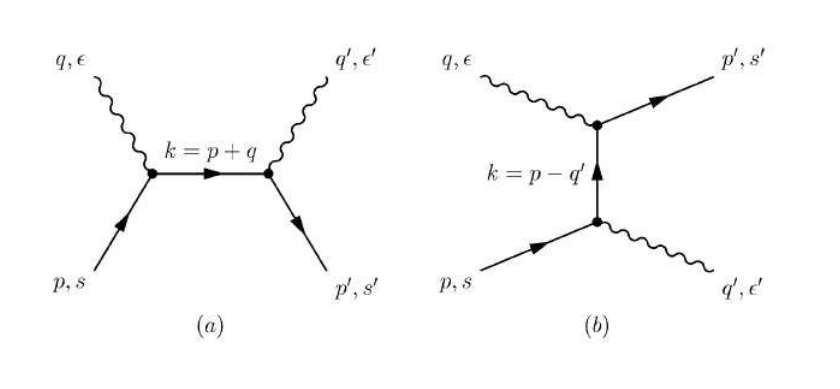
\includegraphics[width=\textwidth]{/home/mitchell/Documents/masters/masters/thesis/Ver_2/figures/Feynman-diagrams-for-Compton-scattering.png}
%\feynmandiagram [horizontal=f2 to f3] {
%  f1 [particle=\(e^{-}\)]-- [fermion] f2 -- [fermion] f3 -- [fermion] f4 [particle=\(e^{-}\)],
%  f2  -- [photon] p1 [particle=\(\gamma\)],
%  f3 -- [photon] p2 [particle=\(\gamma\)],
%};
\label{fig:compton_scattering}
\caption{(a) S-Channel Feynmann Diagram, and (b) T-Channel Feynmann Diagram for Compton Scattering }
\label{fig:compton_scattering}
\end{figure}


It was first described in the context of X-rays interacting with electrons in atoms \citep{1923PhRv...21..483C}, and so regular Compton Scattering is taken to describe the interaction between a high energy photon, and a low energy particle. By applying principles of conservation of momentum, and conservation of energy,  the formula for the shift in wavelength as a result of this scattering is given by
\begin{equation}
	\Delta \lambda = \frac{h}{m_ec}\left(1-\cos\theta\right)
	\label{eqn:compton_shift}
\end{equation}
where $m_e$ is the mass of the electron, and $\theta$ is the angle between the incident and scattered trajectories. 

However, for the SZ effect that is observed in the CMB, the energies of the photons in question are much lower than the energies of the electrons involved, so the frequency shift is parametrised by something called the Compton-$y$ parameter. The expression given by \eqref{eqn:compton_shift} is functional for a single interaction, but given the number of interactions and the statistical nature of the CMB, we have to consider the more broad Compton-$y$ parameter, which is given by:
\begin{equation}
y = \int \frac{k_B T_e}{m_e c^2} n_e \sigma_T d \mathit{l}
\label{eqn:y_param}
\end{equation}
where $m_e c^2$, $k_B$, and $\sigma_T$ are the electron rest mass energy, Boltzmann constant, and Thompson Cross Section respectively. These are all well defined constants, and so have no effect on the integration. 

\par The $y$-parameter therefore amounts to the line-of-sight integration over $n_e T_e$, which are the electron gas density and temperature. The degeneracy between temperature and pressure can be broken in principle by obtaining measurements of one of the two quanties, which we take from hydrodynamical simulations.

This $y$ parameter can be calculated in the CMB from frequency and intensity information at those frequencies. Starting from Kompaneets equation \citep{1957JETP....4..730K}, the time rate of change of the photon occupation number $\bar{n}$ due to Compton Scattering by non-relativistic, isotropic Maxwellian electron gas is given by a non-relativistic Fokker-Planck Equation, \citep{1995ARA&A..33..541R}
\begin{equation}
\pdv{\bar{n}}{t} = \frac{kT}{mc} \frac{\sigma_T n_e}{x^2} \pdv{x} \left[ x^4 \left( \frac{T_e}{T} \pdv{\bar{n}}{x} + \bar{n} + \bar{n}^2 \right) \right],
\label{eq:fk_plnck}
\end{equation}
where $x = h \nu / k T$ is the non-dimensional frequency, $T$ is the temperature of the radiation, $n_e$ and $T_e$ are the number density and temperature of the electrons, and $\sigma_T$ is the Thompson cross section. Because $T_e >> T$, the first term in the parenthesis dominates, reducing the above to 
\begin{equation}
\pdv{\bar{n} }{t} = \frac{k T_e}{m c} \frac{\sigma_T n_e}{x^2} \pdv{x} \left(x^4 \pdv{\bar{n}}{x} \right).
\label{eq:reduced_fk_plnck}
\end{equation}
Since the incident radiation is only weakly scattered, an approximate solution to \ref{eq:reduced_fk_plnck} can be found by substituting the occupation number of a Planckian radiation field
\begin{equation}
\bar{n_p}(x) = \frac{1}{e^x - 1},
\label{eq:plnk_occupation_no}
\end{equation}
By integrating this along a given path length, we can determine the change in spectral intensity along that path, and therefore obtain the spectral form of the SZ effect:
\begin{equation}
g(x) = \frac{x^4 e^x}{(e^x-1)^2} \left[ \frac{x (e^x+1)}{e^x -1 } - 4 \right].
\label{eq:spec_form_y}
\end{equation}

The shape of \eqref{eq:spec_form_y} is shown in Figure \ref{fig:sz}, illustrating how relative frequencies must be rescaled to extract the Compton-$y$ parameter. This spectral form assumes that all the velocity flow of the cluster is given by the thermal energy of the particles, and so there is often a distinction made between the thermal SZ effect (tSZ) and the kinetic SZ effect (kSZ). 
\begin{figure}[h!]
\centering
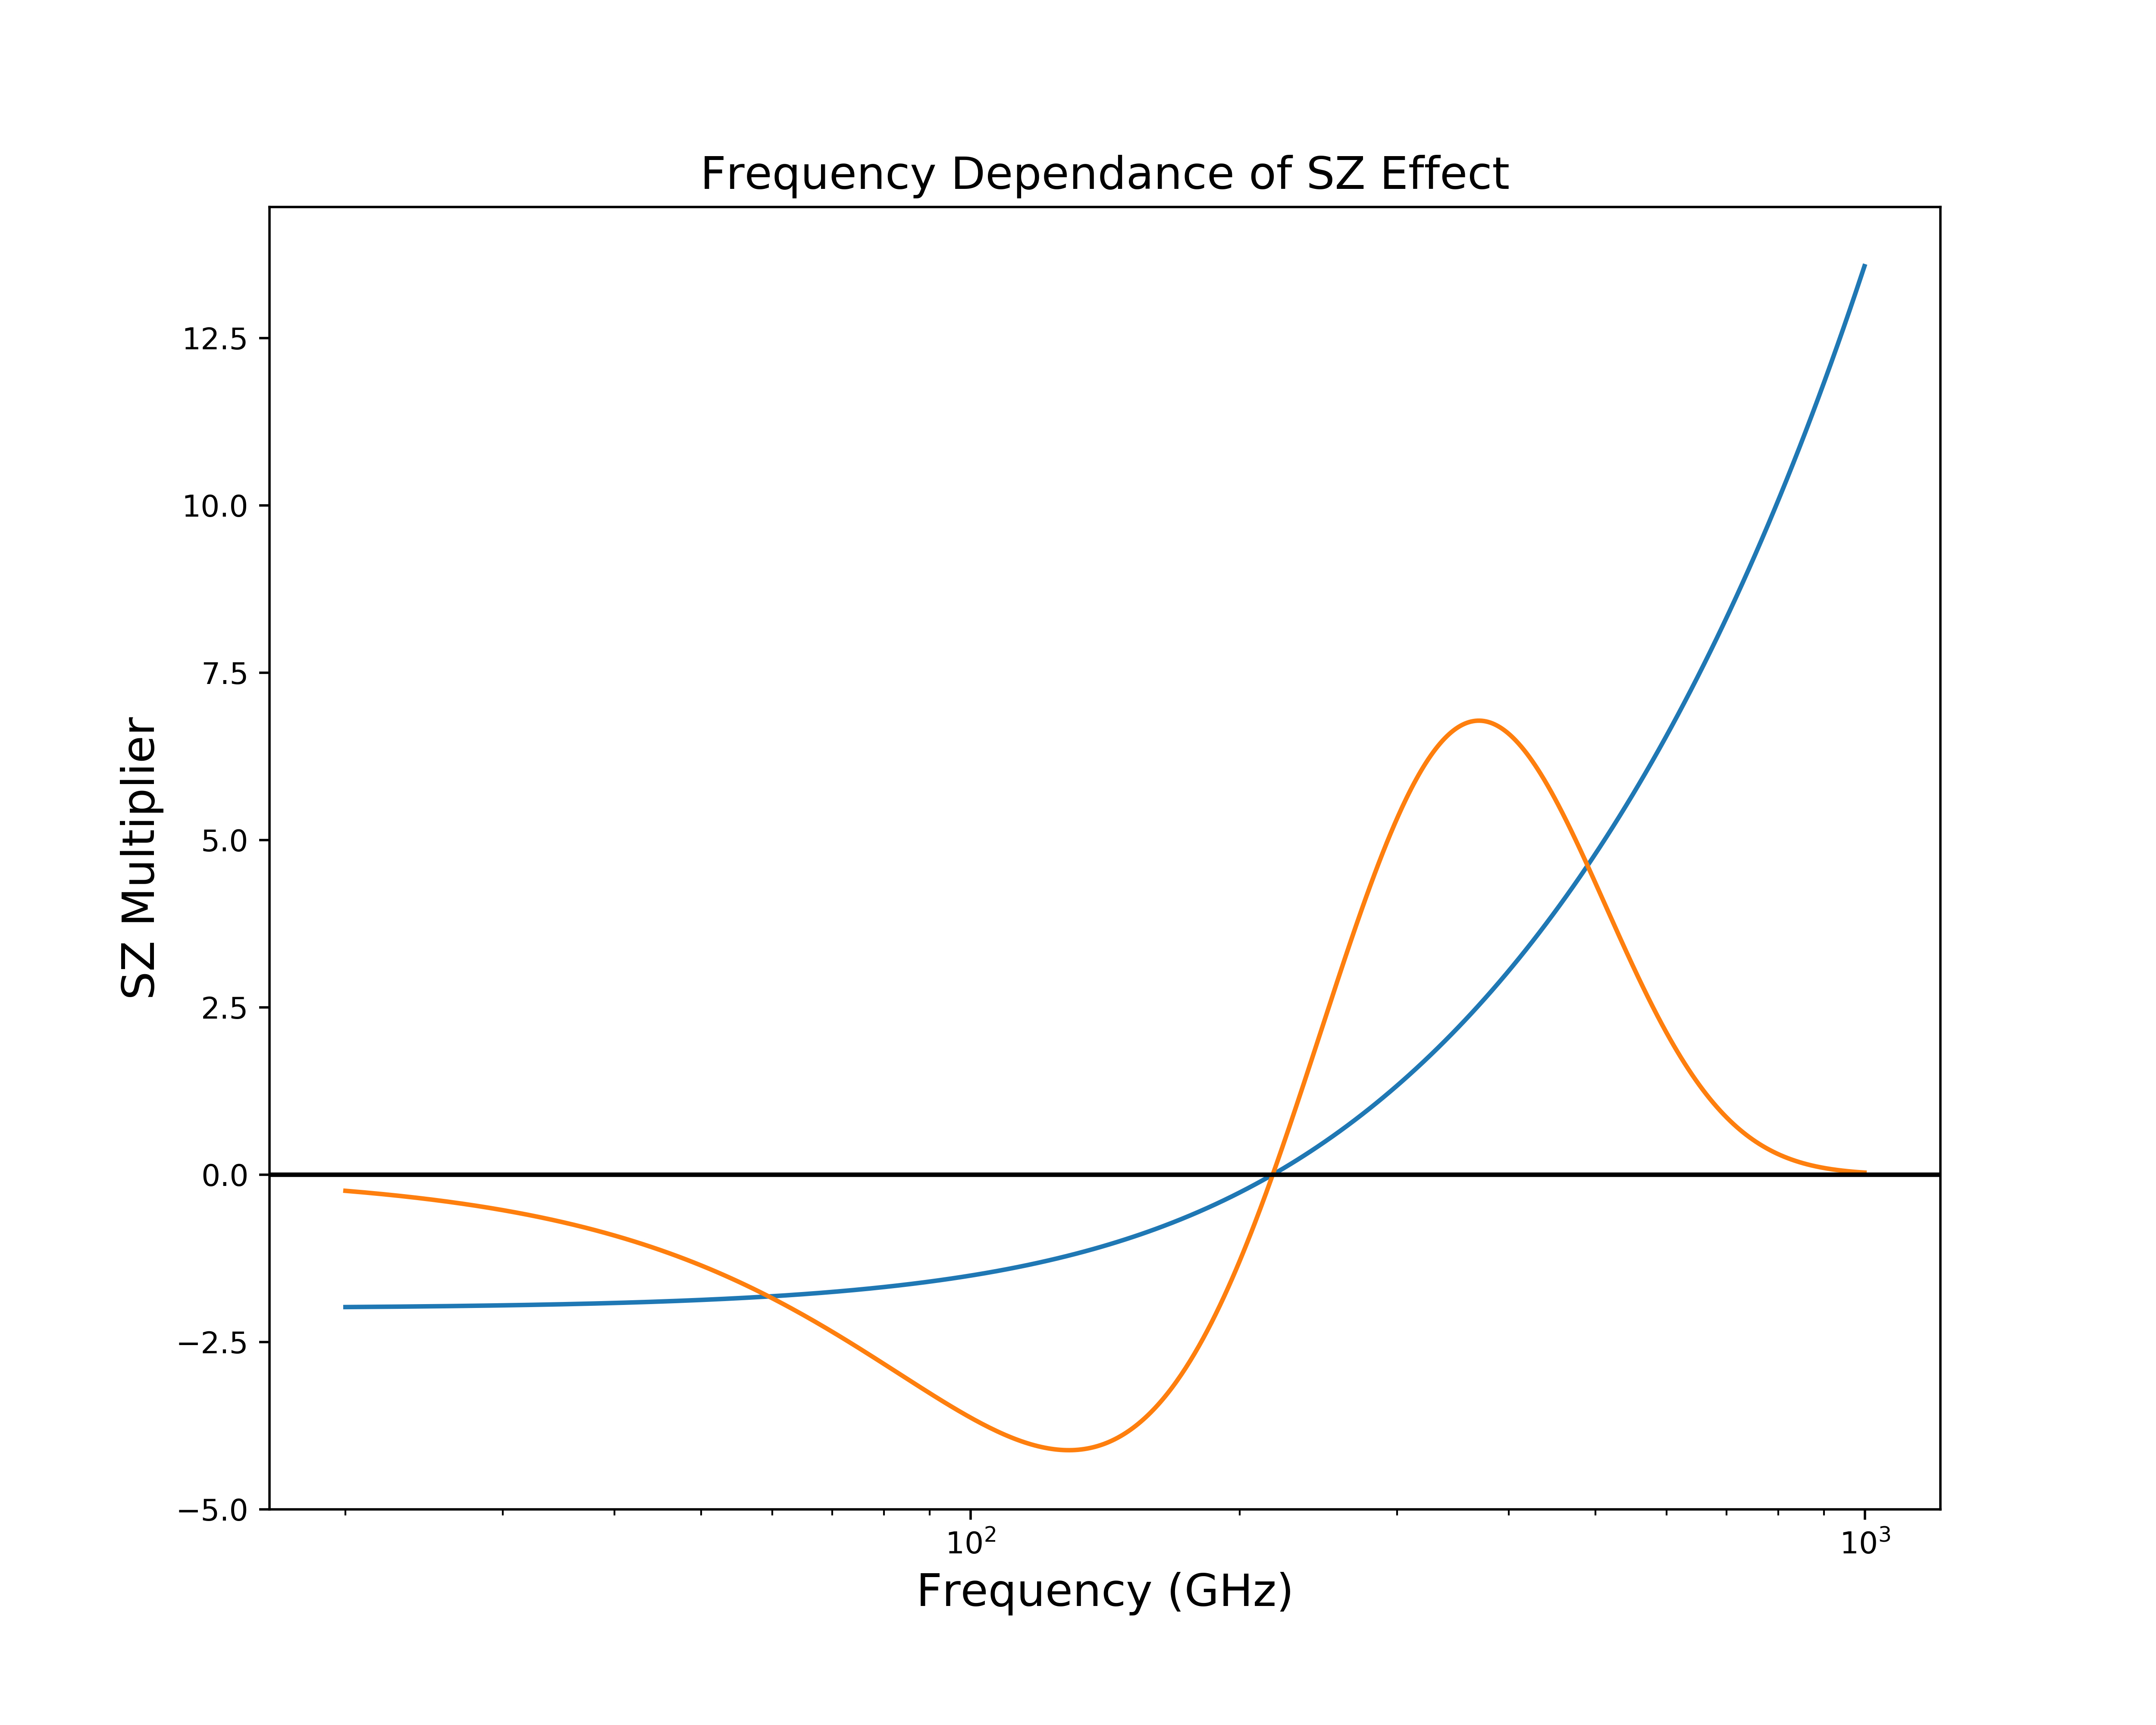
\includegraphics[height=0.4\textheight , keepaspectratio]{/home/mitchell/Documents/masters/masters/thesis/Ver_2/figures/sz_freq.png}
\caption{\sze Intensity and Frequency Scaling Factors}
\label{fig:sz}
\end{figure}

\subsection{CMB Signal}

The method for constructing a map of the SZ effect is given by variants on the 'Internal Linear Combination' (ILC) method \citep{2011MNRAS.410.2481R}. This method presumes very little about the form of the data itself, assuming that it can be written in the form 
\begin{equation}
\vec{x}(p) = \vec{a} s(p) + \vec{n}(p),
\label{eq:ilc_1}
\end{equation}
where $\vec{x}$ is a vector of $N_{obs}$ observations, $s(p)$ is a single map, $\vec{a}$ is a mixing vector, which does not depend on $p$ but is known, and $\vec{n}$ is some noise term, containing both instrument and astrophysical noise. It is also assumed that the maps are the same resolution.

The method then provides an estimator of the mean map, $\hat{s}_{ILC}(p)$ of the map $s$, by making a linear combination $\hat{s}(p) = \vec{w} \vec{x}(p)$:
\begin{equation}
\hat{s}_{ILC} = \frac{\vec{a^t} \hat{R^{-1}}}{\vec{a^t} \hat{R^{-1}} \vec{a}} \hat{x}
\end{equation}
where $\hat{R}$ is the covariance matrix of the observations. 

This method then allows for the map be linearly added together in such a way the the variance is minimised, and so the resulting map is as close to the best fit as possible. 
\par One main advantage of the ILC component separation method is that it doesn't assume a model for the components that are not under direct consideration, they are simply collected in a catch-all nusiance term $\vec{n}(p)$. Unfortunately, if any of these components are correlated with the signals we are looking for, this method is unable to directly separate the signal from the noise without some a priori knowledge of the components $a_i$.

An updated version of the algorithm, known as the modified internal linear combination algorithm (MILCA) \citep{2013A&A...558A.118H}, takes into account three changes to the above methodology. It accounts for localisation in pixel and spherical harmonic spaces to take into account variations in spatial spectral laws. These laws describe the behaviour of different processes at different frequencies, and so are very important to consider when adding maps taken at different wavelengths. It also modifies the definition of the variance being minimised by an action of the covariance matix, to account for the possible correlation between noise and astrophyiscal sources.

Now, this technique can be applied to both the CMB as a whole, as well as the SZ effect specifically, because the characteristic scale and frequency dependance of the SZ is well known.  The size of the anisotropy caused by the SZ effect can be determined from the number of clusters sampled from the observational beam. A detector beam is essentially an instrument's response to the patch of sky it is measuring. It is unique to each instrument, and is a function which convolves everything within its detecting area, effectively smoothing out areas of the sky smaller than its characteristic size.

\par The size of the anisotropy is therefore highly dependant on the constraints on cluster evolution and their subsequent properties. The range of angular scales depends on the angular extent of the clusters, but ultimately sits within ranges of approximately $\SI{1}{\arcmin} - \SI{10}{\arcmin}$ , for a typical cluster with a radial extent of approximately $0.5 h_{-1} $Mpc, and a mass of $2\times 10^{15} M_\odot$. For this system, we expect that the size of the anisotropy to be roughly $\Delta T/T \approx 10^{-6} - 10^{-5}$ \citep{1995ARA&A..33..541R}. This makes sense, since the upper measure for the total comptonisation of the CMB is only $y \approx 4\times 10^{-3}$. However, it does pose an issue for detecting the WHIM, since the average density of a filament is so much lower than the density of a cluster. Since the $y$ parameter is sensitive to the temperature of the gas and the number density, reducing the number density by a factor of $10^5-10^8$ and the gas temperature by $\sim 10^2$, will result in a corresponding reduction in the measured $y$ parameter. 

Given the signal-to-noise ratio expected for the thermal \sze of a single filament, many such filaments must be co-added, so as to drive the signal-to-noise to a detectable level. Initially outlined in \cite{2016MNRAS.457.2391C} for application to weak gravitational lensing maps, it was found that stacking $\sim 135,000$ pairs yielded a filament mass at $\sim 4.5 \sigma$ confidence. Further follow up using the Canada France Hawaii Telescope Lensing Survey (CFHTLenS), and the Sloan Digital Sky Survey's (SDSS) Luminous Red Galaxy (LRG) catalogue by \cite{2017MNRAS.468.2605E} detected the weak lensing signal from stacked filaments at 5$\sigma$ confidence.

Investigations by \cite{2014PhRvD..89b3508V}, \cite{2015JCAP...09..046M}, and \cite{2015JCAP...10..047H} established firmly that there is a correlation between weak gravitational lensing from CFHTLenS and tSZ signals from \emph{Planck}, which suggests that we can use tSZ in the same way as weak lensing, without having to be careful about the peculiarities assosciated with weak lensing, such as sufficiently nulling spherical components. This was further reinforced by \cite{2014JCAP...02..030H}, who reported a $6.2 \sigma$ correlation between the \emph{Planck}  lensing potential and the \emph{Planck}  tSZ map. 
